\section{Intermolecular forces}
Intermolecular forces influence a variety of the physical properties of substances, the most notable of which is their melting and boiling points. Also, if a substance sublimes, it is because the intermolecular forces are extremely weak. There are three types of intermolecular forces.

\subsection{London forces}
These are attractive forces which happen between temporary and induced dipoles, and happen in all molecules. Because of electron oscillation, at any given moment one side of an atom will be electronegative while the other side will be electropositive by a very small amount (as more electrons will be on one side of the molecule). This is called a temporary dipole. These temporary dipoles induce similar dipoles in the surrounding molecules, and as such the dipoles will cause the molecules to have a small electrostatic attraction. As the number of electrons increases, the strength of London forces also increases, as the number of electron oscillations increase and so it is more likely for the molecule to have a stronger temporary dipole.

\subsection{Permanent dipole-dipole interactions}
These are attractive forces that happen between permanent dipoles in polar molecules. The permanent dipole in one molecule attracts the permanent dipole fo another. Substances that have permanent dipole-dipole interactions often have higher boiling points than those that don't as there is extra energy required to overcome them.

\subsection{Van der Waal's forces}
This is an old term that just refers to both London forces, and also to permanent dipole-dipole interactions.

\subsection{Hydrogen bonding}
This is a strong intermolecular force, that happens in covalent molecules which have extremely electronegative atoms (O, N, or F) with lone pairs, and also hydrogens. The interactions happen between the $\delta^+$ at the hydrogens, and the lone pairs of the electronegative atoms in other molecules. An example would be water.
\begin{figure}[h]
	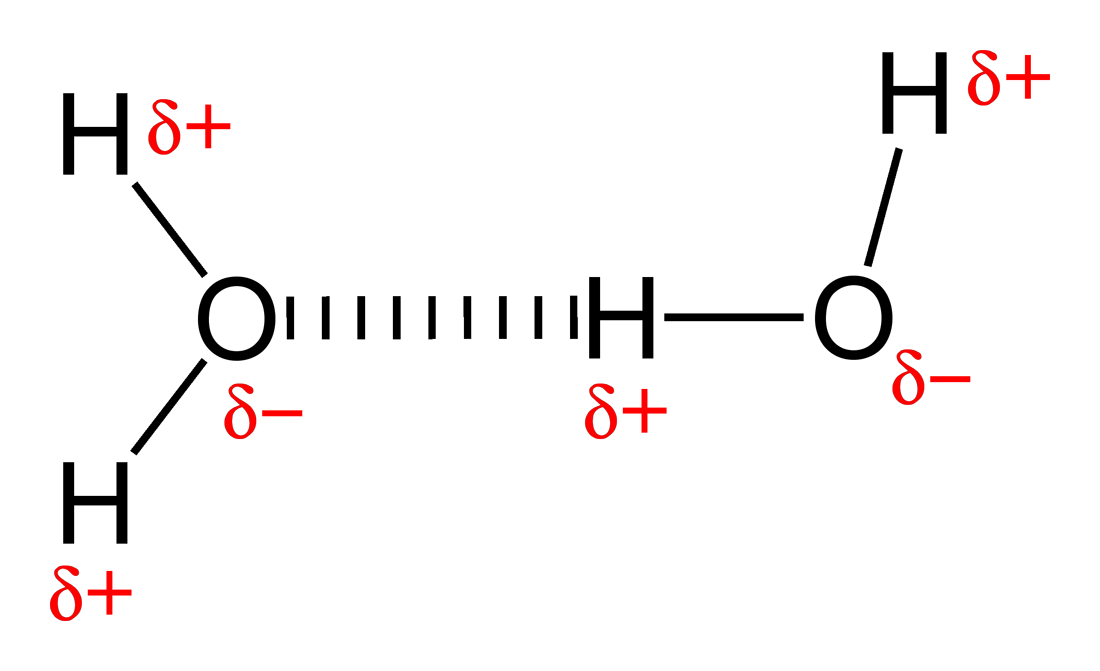
\includegraphics[scale=0.2]{Hydrogen-bonding-in-water-2D}
	\centering
	\caption{An example of hydrogen bonding in water. Image from wikipedia.}
\end{figure}
